
\newpage
\subsubsection{Klimakammer}
\label{subsec:Klimakammer}
\begin{figure}[htb]
\centering		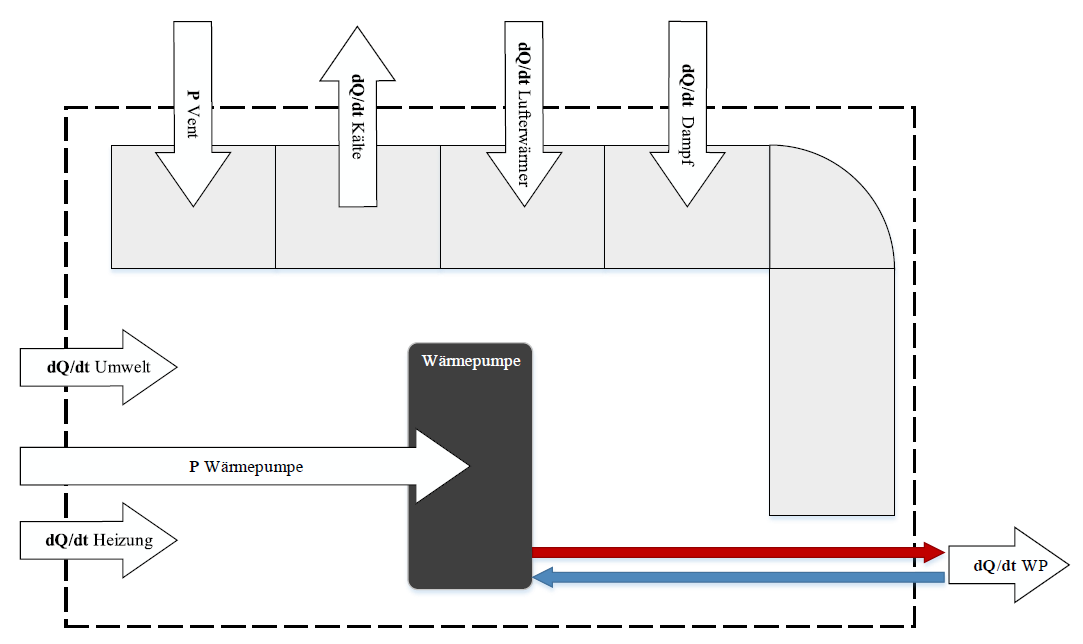
\includegraphics[width=0.850\textwidth]{Pictures/HIL2.png}
\caption{Wärmeströme in der Klimakammer \citep{Nuerenberg2015}}
\label{fig:KK}
\end{figure}


Die Klimakammer erlaubt es, den Verdampfer und somit den Vereisungs- und Abtauprozess unter verschiedenen Abtaubedingungen zu untersuchen. Die Klimakammer ist als klassisches \textit{Hardware in the Loop}-System entworfen und wird so betrieben.  Die Kenndaten der Klimakammer stehen in Tabelle \ref{tab:Parameter KK}. Die Abbildung \ref{fig:KK} zeigt die Wärmeströme innerhalb der Klimakammer. Die Klimakammer ist in der Lage, eine stationäre Umgebungsbedingungen abzubilden. Es ist aber auch möglich, instationäre Situationen wie zum Beispiel Typtage oder -wochen nachzustellen. 
In der Klimakammer ist die Verdampfereinheit mit der Kältemittelversorgungsmimik lokalisiert. Des Weiteren sind das Wägesystem und die eingesetzten Waagen in der Klimakammer platziert. 



Die Klimakammer ist konzipiert für  Untersuchungen von Wärmepumpen und Kältemaschinen. Der Einsatz der Klimakammer in Kombination mit einer klimatisierbaren Versuchshalle hebt die Reproduzierbarkeit von Messungen. Die Bedingungen für Versuche können unabhängig von der Jahreszeit oder dem Tagesklima konstant gehalten werden. So lassen sich Versuche mit verschiedensten Umgebungsbedingungen ganz jährlich durchführen.  Die einzustellenden Parameter sind die Temperatur und die relative Luftfeuchtigkeit ($RH$). Die Klimakammer wurde 2015 in Betrieb genommen und wird wie die Kälteanlage auch über eine SPS der Fa. Beckhoff geregelt und gesteuert. In dem Klimakammer-Projekt wurde von \textsc{\citeauthor{Nuerenberg2015}} beispielsweise die \textit{Statusmaschine} eingeführt, auf der auch das Konzept der SPS der Kälteanlage beruht (siehe Abschnitt \ref{sec:Informationstechnischer Aufbau}). 

Die Klimakammer verfügt über Software-Schnittstellen  mit Simulationssoftware (zB. \textsc{Dymola}) und Datenbanken (zB. \textsc{MySQL}). Die Kombination aus Simulator mit echter Hardware wird als \textit{Hardware in the Loop} bezeichnet. Diese Methode dient zum Testen und Absichern von eingebetteten Systemen, die noch in der Entwicklung sind oder sich in der Inbetriebnahme befinden. Die Vorteile dieser Methode liegt in der Verkürzung der Inbetriebnahmephase, Verringerung der Entwicklungskosten und im risikofreien Testen der Anlage in Grenzsituationen. \citep{OPALRTT2014}


\begin{table}[htb]
\centering
\caption{Systemparameter der Klimakammer \citep{Nuerenberg2015}}\vspace{6pt}
\label{tab:Parameter KK}
\begin{tabular}{ll}
\hline 
\textbf{Systemparameter} & \textbf{Klimakammer} \\ 
\hline 
\hline
Volumen & 32,96 m$^3$ \\ 
\hline 
Oberfläche & 74,4 m$^2$ \\ 
\hline 
U-Wert & 0,15 W/(m$^2$K) \\ 
\hline 
max. Volumenstrom & 4000 m$^3$/h \\ 
\hline 
max. Leistung der Lufterwämer & 2x 20 kW \\ 
\hline 
max. Befeuchtungsleistung & 12 kg/h \\ 
\hline 
max. Kühlleistung & 10 kW \\ 
\hline 
min. Temperatur & - 16,8 °C \\ 
\hline 
Steuer- und Regelungstechnik & TWINCAT 3/ VB.NET \\ 
\hline 
Hart echtzeitfähig & Ja \\ 
\hline 
\hline
\end{tabular} 
\label{tab:Systemparameter-KK}
\end{table} 

